\chapter{Electronic Excited States}

\begin{quote}
  "The XXIst century might be very well the century of light. Understanding and controlling photoexcited systems will be crucial for future research in many branches of optics and photonics."
  \begin{flushright}
    \small{--- \textit{L. González, D. Escudero, L. Serrano-Andrés (2011) [Gon2011] }}
  \end{flushright}
\end{quote}


% Gon2011 https://chemistry-europe.onlinelibrary.wiley.com/doi/10.1002/cphc.201100200

\section{Nature of Excited States}

The potential energy landscape of electronic excited states is complex and governed by various absorption and decay mechanisms. Excitations are generally grouped into three categories:
\begin{enumerate}
\item \emph{Valence excitations}, where valence electrons are excited into (local) higher lying unoccupied orbitals above the Fermi level
\item \emph{Rydberg excitations}, where electrons are excited into very diffuse orbitals around the molecule
\item \emph{Charge transfer excitations} (CT), where electrons are excited to different parts of the molecule or different molecules entirely. 
\end{enumerate}
\noindent Furthermore, \emph{core excitations} specify transitions of the core electrons ????

Excited states typically have lifetimes and decay back to the ground state via several different mechanisms. Figure \ref{fig:PESEX} illustrates the different processes. The notation $S$, $D$, $T$ ... is used to denote singlet, doublet, triplet ... states and the subscripts indicate the energy level, where 0 is the ground state, 1 is the first excited state for the given spin symmetry, 2 is the second excited state etc. The transition from the ground state $S_0$ to the excited state $S_1$ on the same reaction coordinate is known as a \emph{vertical excitation}. The excited state may be in a higher vibrational state at that reaction coordinate (indicated by the lines within the potential wells), and relax to the lowest level. The difference between these two points is known as the \emph{reorganization energy}, and the difference between the lowest vibrational states of $S_0$ and the excited state is known as the \emph{adiabatic excitation} energy. The 
molecule returns to the ground state by emitting a photon in a process known as \emph{fluorescence}. 

Surfaces of different states may cross at specific reaction coordinates. The crossing between states with different multiplicity (e.g. S$_1$ tp T$_1$) is known as an intersystem crossing (ISC). The process between two states where the crossing takes place between molecules of the same spin-symmetry is known as \emph{internal conversion} (IC), and takes place at a \emph{conical intersection} (CoIn). The S$_1$ excited state can cross over to the T$_1$ state via an ISC which then decays in a process known as \emph{phosphorescence}, or it can decay radition-less via the CoIn. 

At the ISC and CoIn, the Born-Openheimer approximation breaks down and processes that occur via surface crossing are governed by \emph{non-adiabatic} dynamics...... 

\begin{figure}
\centering
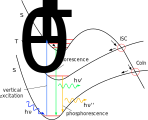
\includegraphics[scale=0.8]{Pics/PESEX}
\caption{Potential energy surface}
\label{fig:PESEX}
\end{figure}

\section{Explicit Optimization of the Excited State Wavefunction}

One of the conceptually simplest approaches for obtaining information on excited states is explicit optmization of the excited wavefunction. The excitation energy is then directly computed by taking the difference between the ground state energy and the energy of excited state $i$
\begin{equation}
E_{0\rightarrow i} = E_i - E_0 
\end{equation} 
\noindent Any ground state model discussed in the previous chapter can be used. This approach to excited states is known by different names, depending on which approximation is used. Generally, the greek letter $\Delta$ is just prepended to the method name, giving $\Delta$SCF or $\Delta$HF for Hartree-Fock (21,22,myself), $\Delta$KS (Kohn-Sham) or $\Delta$DFT for DFT (25,26,27), and so on. At the moment of writing, excitation energies are also routinely computed using $\Delta$MP$n$ (23), $\Delta$CI, $\Delta$MCSCF (24) and $\Delta$CC (23,a). From here on out, $\Delta$X will be used as an umbrella term to group all aforementioned terms. 

Depsite the simplictly of the $\Delta$X methods, obtaining a solution to the KS or HF equations for higher energy states is non-trivial. By the variational principle, the SCF method finds the lowest energy solution. A HF type excited wavefunction may theroefore collapse to that lowest energy solution during the SCF procedure (variational collapse). This technical difficulty was one of reasons why $\Delta$X methods never gained much ground compared to more sphisticated methods.

In 2008, Gilbert et al. (ref) proposed a modification the SCF procedure that prevents variational collapse, known as the \emph{maximum overlap method} (MOM). On each iteration, the new guess orbitals are obtained by diagonalization of the Fock matrix which is constructed using the old coefficients
\begin{equation}
\mbf{F}(\mbf{C}^{old})\mbf{C}^{new} = \mbf{S}\mbf{C}^{new}\epsilon
\end{equation}
\noindent At this step, it is possible to decide which of those new orbitals are actually occupied. Normally, the $n_{occ}$ eigenvectors with the lowest eigenvalues are chosen as the new occupied MOs. Alternatively, the MOM protocol chooses the set of new MOs that overlap most with the span of the old coefficients, by evaluating the overlap matrix
\begin{equation}
\mbf{O} = (\mbf{C}^{old})\pdg \mbf{C}
\end{equation}

The maximum overlap method has led to a renewed interest in the $\Delta$X methods in recent years, especially in the context of core excitations and ionizations (see below). 

In the additon to the above-mentioned technical difficulties, there are several other known criticisms. First, each excited state requires a separately optimized wave function, which may become a limiting factor. Second, the $\Delta$X methods assume that a transition can be represented by an excitation involving two orbitals. The separate optimization generally leads to the excited states being non-orthogonal, and there is considerable overlap between high and low energy states (39-41). $\Delta$X is therefore assumed to be only applicable to low-lying excited states (42). Third, the transition moments cannot be computed directly, but need to be evaluated using Fermi's Golden Rule (44). Futhermore, to allow a comparison with experimenatl XAS spectra, the calculated transition energies must be  convoluted by for example Gaussian functions to 
account for the finite experimental resolution and  lifetime of the electron hole. Finally, using an unrestricted HF or KS formalism leads to spin contamination. A single excited state is not a pure singlet but a mixture of singlet and triplet state. Spin contamination can be alleviated by applying Ziegler's spin purification formula (45):

\begin{equation}
E_S = 2 E_{mixed} - E_T
\end{equation}

Despite these disadvantages, $\Delta$X has been shown to be an attractive and low-cost alternative to response and propagator methods.

a doi:10.1021/acs.jctc.9b00568 

\section{Time-depedenent stuff??}

\section{The Algebraic Diagrammatic Construction Method}

The algebraic diagrammatic construction (ADC) scheme is an excited state method originating from Green's functions. By diagrammtic perturbation expansion of electron propagators, ADC gives a hierarchy of methods which sytematically converge to the exact solution (Full CI).  

\subsection{Many-Body Green's Function}

Many-Body Green's Functions (MBGFs) are powerful tools to treat electron correlation in quantum mechanics. They are more commonly encountered in (condensed matter) physics, for the modelling of strongly correlated systems such as metals or semi-conductors. MBGFs get their name from their building blocks: Green's functions (GFs). GFs, or \emph{correlation functions}, are special solutions to differential equations (DEQs).

Consider the inhomogenous DEQ in one dimension:
\begin{equation}
\hat{D}_x y(x) = f(x)
\end{equation}
\noindent where $\hat{D}$ is a linear differential operator. The general solution can be divided into a \emph{homogenous} and a \emph{special} part
\begin{equation}
y(x) = y_{hom}(x) + y_{spec}(x)
\end{equation}
\noindent where $y_{hom}$ is the solution to the homogenous equation $\hat{D}y_{hom}(x)$ = 0. The special solution can be expressed in terms of GFs which are defined as the solution to the DEQ where the inhomogeneity is a Dirac function:
\begin{equation}
\hat{D}_x G(x,x') = \delta(x-x')
\end{equation}
\noindent A special solution can then be constructed by
\begin{equation}
y_{spec} = \int G(x,x')f(x') dx
\end{equation}
\noindent for any inhomogeneity $f(x)$. 

The Schrödinger equation is also a differetial equation where the inhomogeneity takes the role of the external perturbation $V$
\begin{equation}
\left[ i\frac{\partial}{\partial t} + \frac{1}{2} \nabla^2 \right] \Psi(\mbf{r},t) = V(\mbf{r},t) \Psi(\mbf{r},t)
\end{equation}
\noindent The wave function may then be expressed by
\begin{equation}
\Psi(\mbf{r},t) = \int G(\mbf{r},t;\mbf{r}',t') \Psi
\end{equation}
\noindent The GF has the effect of \emph{propagating} the wave function from a given time and position to another time and spce coordinate. GFs are therefore also known as \emph{propagators}.

The MBGFs form a hierarchy, in which the one-particle GFs are the lowest rank (Figure \ref{fig:PROP}). One-particle GFs can be used to extract information on 1-electron processes such as ionization and electron attachment. Two-particle GFs form the next step in the hierarchy, and allow to gain infomation on two-particle processes such as electron excitation (electron-hole) and two-electron ionization (electron-eletron). 
\begin{figure}
\centering
\includegraphics[scale=0.6]{Pics/PROP}
\caption{A caption}
\label{fig:PROP}
\end{figure}

\subsubsection{One-electron Propagator}

To see how GFs can be used for excited state analysis, consider the 1-electron propagator in the time domain
\begin{equation}
G_{pq}(t,t') = - i\Theta(t-t') \sbra{\Psi_0} \hat{T}(a_p[t]a
_q\pdg[t']) \sket{\Psi_0}
\end{equation}
\noindent where $\Theta$ is Heavyside step function, and with the time-ordering operator 
\begin{equation}
\hat{T} = \left\lbrace \begin{matrix}
a_p[t] a_q\pdg[t'] \quad \textrm{for } t > t' \\
-a_q\pdg[t'] a_p[t] \quad \textrm{for } t < t'
\end{matrix}
\right.
\end{equation}
\noindent which plays the role of conserving symmetry with respect to time. It is useful to switch to the energy representation of the GF by Fourier transformation
\begin{equation}
G_{pq} (\omega) = \underbrace{ \sum_n \frac{
	\sbra{\Psi_0} c_p \sket{\Psi_n^{N+1}}			    \sbra{\Psi_n^{N+1}} c_q \pdg \sket{\Psi_0} 
}{
	\omega + E_0 - E_n^{N+1} + i \eta
}
}_{\text{$G^{+}(t,t')$}} + 
\underbrace{
\sum_n \frac{
	\sbra{\Psi_0} c_q \pdg \sket{\Psi_n^{N-1}}			    \sbra{\Psi_n^{N-1}} c_p \sket{\Psi_0}
}{
	\omega + E_n^{N-1} - E_0 - i \eta
}
}_{\text{$G^{-}(t,t')$}}
\end{equation}
\noindent also known as the spectral or Lehmann representation. The superscripts $N+1$ and $N-1$ indicate the addition or removal of an electron form the $N$-electron wave function. The left-hand sum $G^{+}$ describes electron attachment and the right-hand term $G^{-}$ describes electron detachment (ionization). The singularities or \emph{poles} of the spectral representation give the $n$th electron affinity and ionization energy 
\begin{align}
A_n &= E_0 - E_n^{N+1} \\
I_n &= E_n^{N-1} - E_0
\end{align}
\noindent Moreover, the transition strengths (or pole strengths) are given by the spectroscopic factors 
\begin{equation}
x_p^{(n)} = \bra{\Psi_0 } c_p \ket{\Psi_n ^{N+1} }, \quad n \in \left\lbrace N + 1 \right\rbrace
\end{equation}
\begin{equation}
x_p^{(n)} = \bra{\Psi_n^{N-1} } c_p \ket{\Psi_0 }, \quad n \in \left\lbrace N - 1 \right\rbrace
\end{equation}
\noindent By analysing the 1e-GF, it is therefore possible compute the 1-particle excitation spectrum. 

\subsubsection{Polarization Propagator}

A solution to the single-particle SEQ can be given directly by integrating the GFs. For many-electron systems however, one- and two-particle GFs are only building blocks for many-body propagators. The 1p and 2p GFs allow to introduce the particle-hole response function (ref1) 
\begin{equation}
R_{pq,uv}(t_1,t_2;t_1',t_2') = G_{pq,uv}(t_1,t_2;t_1',t_2') - G_{pu}(t_1,t_1')G_{qv}(t_2,t_2')
\end{equation}
\noindent also known as the two-particle correlation function. It is the variational derivative of the 1p-GF with respect to an external perturbation $V(t_1,t_2)$, for example an incoming light quantum (Bay1962). Similarly to the 1p-GF, analyzing the ph response function gives information on the excited state. It can be evaluated directly via the Bethe-Salpeter equations (ref), but the dependence on four time variables make them difficult to solve. The same information is already contained in the \emph{polarization propagator} defined by
\begin{equation}
\Pi(t,t') = \lim_{\substack{t_1 \rightarrow t_1'=t \\
t_2 \rightarrow t_2' = t'}} iR(t_1,t_2;t_1',t_2')
\end{equation}  
\noindent The spectral representation of $\Pi$ takes the form
\begin{equation}
\Pi _{p,q;r,s} = \underbrace{ \sum_{n \neq 0} \frac{ 
	\bra{\Psi_0} \hat{c}_q \pdg \hat{c}_p 		\ket{\Psi_n} \bra{\Psi_n} \hat{c}_r \pdg \hat{c}_s \ket{\Psi_0}
}{
	\omega - (E_n - E_0) + i \eta
} }_\text{$\Pi _+(\omega)$} + \underbrace{ \sum_{n \neq 0} \frac{ 
	\bra{\Psi_0} \hat{c}_r \pdg \hat{c}_s \ket{\Psi_n} \bra{\Psi_n} \hat{c}_q \pdg \hat{c}_p \ket{\Psi_0}
}{
	- \omega - (E_n - E_0) + i \eta
} }_\text{$\Pi _-(\omega)$}
\label{eq:POLPROP}
\end{equation}
\noindent Here, the poles correspond to the excitation energies $\omega_n = E_n - E_0$ and the spectroscopic factors give the transtion strengths. The polarization propagator is therefore all one needs to evaluate absorption or emission spectra of molecules. The left and right hand terms are related by
\begin{equation}
\Pi(-\omega)_{+}\pdg = \Pi_{-}(\omega)
\end{equation}

Up to this point, the exact wave function was used in the expression for the propagators. To actually be able to compute the propagtors, one needs to introduce approximations. There are a couple of choices. Coupled cluster linear response theory inserts the CC ansatz for the wave fucntion and explicitly evaluates expressions for the polaization propgator truncated to a given level of excitations (LR-CCSD, LR-CCSDT etc.).

Alternatively, the polarization propagator may be approached using perturbation theory.

\subsubsection{Diagrammatic Perturbation}

Similarly to the wave function in RSPT, the polarization propagator can be expanded as
\begin{equation}
\Pi = \Pi^{(0)} + \Pi^({1}) + \Pi^{(2)} + \ldots
\label{eq:PERTPOLPROP}
\end{equation}
\noindent The same partitioning of the Hamiltonian is used as previously
\begin{equation}
\hat{H} = \hat{H}_0 + \hat{U}
\end{equation}
\noindent with the expressions for the wave functions and their energies given in Equations ... and ... 

One may then evaluate the series \ref{eq:PERTPOLPROP} using either Rayleigh-Schrödinger perturbation theory or the Gell-Mann Low theorem (ref) to obtain master equations for $\Pi^{(n)}$. However, these eqautions are very tedious to solve, even more so than for M{\o}ller Plesset, due to the rapidly increasing number of nested terms for higher $n$. For this reason, diagrams were introduced to better keep track of the contributions at a given level. 

Diagrams were orginally conceived by Feynman, and are a pictorial representation of mathematical expressions for particle interactions. Over the years, many different types of diagrams were proposed, such as Goldstone, Abrikosov or Hugenholtz diagrams. Each type has its own set of rules on how to construct them and translate them into formulas for a given problem. There is no formal proof: Feynman first worked out the rules by trial and error (Fey1966), and later refined the model.

% Bay1962 https://journals.aps.org/pr/abstract/10.1103/PhysRev.127.1391
% Sal1951 E. E. Salpeter and H. A. Bethe, Phys. Rev. 84, 1232 (1951)
% Fey1966 https://science.sciencemag.org/content/153/3737/699

Figure ... shows the Feynman diagrams (in Abrikosov notation) for the polarization propagator up to second order. 

\subsection{The ADC scheme}

The polarization propagator cannot be directly "measured". To establish a bridge between theory and experiments, the \emph{transition function} is introduced as
\begin{equation}
T(\omega) = D\pdg \mbf{Pi}_{+} D 
\end{equation}
\noindent where $\hat{D}$ is an arbitrary operator. The quantity measured during experiments is the \emph{spectral function}, given by
\begin{equation}
f(\omega) = \frac{1}{\pi}Im\{T(\omega)\}
\end{equation}
In the algebraic diagrammatic construction method, the transition function is reformulated as
\begin{equation}
T(\omega) = \mbf{F}\pdg \mbf{\Gamma}(\omega) \mbf{F}
\end{equation}
\noindent where $\mbf{F}$ are the modified transition moments and the non-diagonal matrix $\mbf{\Gamma}$ is given by
\begin{equation}
\mbf{\Gamma}(\omega) = \left[ \omega \mbf{1} - (\mbf{K} + \mbf{C}) \right] = \left[ \omega \mbf{1} - \mbf{M} \right]
\end{equation}
\noindent whith the ADC matrix $\mbf{M}$. Writing the transition function, the modified transition moments and $\mbf{M}$ as a perturbation expansion
\begin{align}
T(\omega) &= \sum_{n=0}^{\infty} T^{(n)}(\omega) = \sum_{n=0}^{\infty} D\pdg \mbf{Pi}_{+}^{(n)} D
\mbf{F} &= \sum_{n=0}^{\infty} \mbf{F}^{(n)} \\
\mbf{M} &= \mbf{K} + \sum_{n=1}^{\infty} \mbf{C}^{(n)}
\end{align} 
\noindent the $n$th order approximations to the transition function read
\begin{align}
T^{(0)}(\omega) &= \mathbf{F}^{(0)\dagger} \left[ \omega \mathbf{1} - \mathbf{K} \right]^{-1} \mathbf{F}^{(0)} \\
\begin{split}
T^{(1)}(\omega) &= \mathbf{F}^{(0)\dagger} \left[ \omega \mathbf{1} - \mathbf{K} \right]^{-1} \mathbf{C}^{(1)} \left[ \omega \mathbf{1} - \mathbf{K} \right]^{-1} \mathbf{F}^{(0)} + \mathbf{F}^{(1)\dagger} \left[ \omega \mathbf{1} - \mathbf{K} \right]^{-1} \mathbf{F}^{(0)} \\
&+ \mathbf{F}^{(0)\dagger} \left[ \omega \mathbf{1} - \mathbf{K} \right]^{-1} \mathbf{F}^{(1)} 
\end{split} 
\\
\begin{split}
T^{(2)}(\omega) &= \mathbf{F}^{(1)\dagger} \left[ \omega \mathbf{1} - \mathbf{K} \right]^{-1} \mathbf{F}^{(1)} + \mathbf{F}^{(0)\dagger} \left[ \omega \mathbf{1} - \mathbf{K} \right]^{-1} \mathbf{C}^{(2)} \left[ \omega \mathbf{1} - \mathbf{K} \right]^{-1} \mathbf{F}^{(0)} \\
&+ \mathbf{F}^{(0)\dagger} \left[ \omega \mathbf{1} - \mathbf{K} \right]^{-1} \mathbf{C}^{(1)} \left[ \omega \mathbf{1} - \mathbf{K} \right]^{-1} \mathbf{C}^{(1)} \left[ \omega \mathbf{1} - \mathbf{K} \right]^{-1} \mathbf{F}^{(0)} \\
&+ \mathbf{F}^{(1)\dagger} \left[ \omega \mathbf{1} - \mathbf{K} \right]^{-1} \mathbf{C}^{(1)} \left[ \omega \mathbf{1} - \mathbf{K} \right]^{-1} \mathbf{F}^{(0)} \\
&+ \mathbf{F}^{(0)\dagger} \left[ \omega \mathbf{1} - \mathbf{K} \right]^{-1} \mathbf{C}^{(1)} \left[ \omega \mathbf{1} - \mathbf{K} \right]^{-1} \mathbf{F}^{(1)}
\end{split}
\end{align}
\noindent By comparing the above $n$th order expression of the transition operator $T(\omega)^{(n)}$ with the expression of $\mbf{D}\pdg \mbf{\Pi}(\omega) \mbf{D}$ derived using the diagrammatic perturbation of the polarization propagator, algebraic expressions can be \emph{constructed} for the transition moments $\mbf{F}$, and the matrices $\mbf{K}$ and $\mbf{C}$. 

The reader is referred to the original paper for a step-by-step derivation (Schirmer). 

\subsection{Structure of the ADC matrix}

The solution to the eigenvalue problem
\begin{equation}
\mbf{M}\mbf{X} = \mbf{X}\mbf{\Omega}
\end{equation}
\noindent yields the vertical excitation energies and the eigenvectors $mbf{X}$. Figure \ref{fig:ADCMAT} shows the structure of the ADC matrix $\mbf{M}$ up to third order. Each second level $n$ adds an additional higher excitation manifold to the matrix. ADC(0) and ADC(1) include only singles, while ADC(2) and ADC(3) also include doubles.

The ADC(0) matrix contains only the Hartree-Fock orbital energy differences:
\begin{equation}
M^{(0)}_{ia,jb} = K_{ia,jb} = \delta_{ij}\delta_{ab} (\eps_i - \eps_a) 
\end{equation}
\noindent The ADC(1) matrix adds the first order expression for $\mbf{C}$, and is identical to the CIS matrix:
\begin{equation}
M^{(1)}_{ia,jb} = K_{ia,jb} + C_{ia,jb}^{(1)} = \delta_{ij}\delta_{ab} (\eps_i - \eps_a) - \sbra{ij}\sket{ab}
\end{equation} 
\noindent The ADC(2) matrix has addtional second order contributions to the p-h block, and approximates the 2h-1p, 1h-2p and 2p-2h contributions up to first order. 
\begin{align}
C_{ijab}^{(2)} &= C_{ijab}^{(2)A} + C_{ijab}^{(2)B} + C_{ijab}^{(2)C} 
\\
C_{ia,jkcl}^{(1)} &= \sbra{kl} \sket{id} \delta_{ac} - \sbra{kl} \sket{ic} \delta_{ad} - \sbra{al} \sket{cd} \delta_{ik} + \sbra{ak} \sket{cd} \delta_{il} 
\\
C_{iajb,kc}^{(1)} &= \sbra{kb} \sket{ij} \delta_{ac} - \sbra{ka} \sket{ij} \delta_{bc} - \bra{ab} \sket{cj} \delta_{ik} + \sbra{ab} \sket{ci} \delta_{jk} 
\\
K_{iajb,kcld} &= (\epsilon_a - \epsilon_i + \epsilon_b - \epsilon_j) \delta_{ac} \delta_{bd} \delta_{ik} \delta_{jl} 
\end{align}

\noindent with

\begin{align}
C_{ijab}^{(2)A} &= \frac{1}{4} \delta_{ij} \sum_{ckl} \left[  \hat{t}_{ackl} \bra{kl} \sket{bc}  +  \bra{ac} \ket{kl} \hat{t}_{klbc}\right] \\
C_{ijab}^{(2)B} &= \frac{1}{4} \delta_{ab} \sum_{cdk} \left[ \hat{t}_{cdik} \bra{jk} \ket{cd} + \bra{cd} \ket{ik} \hat{t}_{jkcd} \right] \\
C_{ijab}^{(2)C} &= - \frac{1}{2} \sum_{ck} \left[ \hat{t}_{acik}  \bra{jk} \ket{bc} + \bra{ac} \ket{ik} \hat{t}_{jkbc} \right] 
\end{align}

and the antisymmetrized MP2 amplitudes

\begin{equation}
\hat{t}_{ijab} = \frac{\sbra{ij}{ab}}{\eps_a + \eps_b - \eps_i - \eps_j}
\end{equation}

\begin{figure}
\centering
\includegraphics[scale=0.4]{Pics/ADCMAT2}
\caption{A caption}
\label{fig:ADCMAT}
\end{figure}

\subsection{Intermediate states}

An alternative route to derive the ADC working eqautions is via the intermediate state representation (refs 55, 63, 77, 78 Andreas). 

The prvious derivation showed that the eigenvalues of the ADC matrix $\mbf{M}$ correspond to the excitation energies, and that it can be expanded in a perturbation series. These features suggest, that $\mbf{M}$ is a representation of the energy-shifted Hamiltonian
\begin{equation}
\mbf{M} = \mbf{H} - E_0
\end{equation}
\noindent with the matrix elements 
\begin{equation}
M_{IJ} = -\sbra{\tPsi_I} \hat{H} - E_0 \sket{\tPsi_J}
\end{equation}
\noindent Here, the space of the shifted Hamiltonian is spanned by a set of \emph{intermediate states}. Starting from the set of \emph{correlated excited} (CE) states
\begin{equation}
\sket{\Psi^{\#}_I} = \hat{C}_I \sket{\Psi_0} 
\end{equation}
\noindent with the excitation operators
\begin{equation}
\{\hat{C}_I\} = \{ a_a\pdg a_i; a_b\pdg a_j c_a\pdg c_i; \ldots \}
\end{equation}
\noindent the intermediate states are obtained by a step-wise Gram-Schmidt orthogonalization of the CE states. The ground state $\sket{\Psi_0}$ is approximted by MPPT. Constructing the ISs from the MP$n$ ground state wave function and evaluating the matrix elements according to ... gives the $n$th order ADC matrix. For this reason, ADC is also known as "excited state method for M{\o}ller-Plesset". 

\subsection{Variants}

\subsection{Performance}

\section{Response Theory}

linear response theory, tddft, tdhf, RPA?

\subsection{Connection between CC2-LR and ADC}

\section{Equation-of-Motion}

\subsection{Connection between EOM and CCLR}


\section{Time-dependent stuff?}